%%%%%%%%%%%%%%%%%%%%%%%%%%%%%%%%%%%%%%%%%%%%%%%%%%%%%%%%%%%%%%%%%%%%%%%%%%%%%%%
%%%  Document settings                                                      %%%
%%%%%%%%%%%%%%%%%%%%%%%%%%%%%%%%%%%%%%%%%%%%%%%%%%%%%%%%%%%%%%%%%%%%%%%%%%%%%%%

\documentclass[11pt,a4paper,twoside,openright]{report}
%% ETHDASA + fancyheadings + sfs-hyper -> hyperref
\usepackage{ETHDAsfs} 
%% to include the confirmation of originality (plagiarism
\usepackage{pdfpages}
%% for \boldsymbol and \pmb{.}
\usepackage{amsbsy}
%% calls  amsfonts...
\usepackage{amssymb}
%% for ps-graphics
\usepackage{graphicx}
%% use 'numbers' : \usepackage[longnamesfirst,number]{natbib} for [1], [2] 
\usepackage[longnamesfirst]{natbib}
%% NOTE: texab contains many useful definitions and "shortcuts". 
%% e.g. \R, \Z, \Q, \Nat for real, integer, rational, natural numbers;
%% \N (normal dist.), \W == probability; \med, \var, \Cov, \abs{x} == |x|
%% and \norm{y} == || y ||
%% Open the file and have a look at them. HOWEVER, some
%% definitions are a bit can lead to conflicts with other packages. You
%% might for example want to comment out the line defininf \IF as an
%% operator when working with the algorithmic package, or to comment out
%% the line defining a command \Cite with working with the Biblatex package  
\usepackage{texab}
\usepackage{amsmath}
%% Raph Smith's Formal Script font --> provides \mathscr
%\usepackage{mathrsfs}
\usepackage{enumerate}
%% \smaller (etc) used here
\usepackage{relsize}
%% to allow cloring in code listings
\usepackage{color}
%% for code blocks
\usepackage{listings}
%% for linenumbers only!
\definecolor{Mygrey}{gray}{0.75}
%% for comments
\definecolor{Cgrey}{gray}{0.4}
\lstloadlanguages{R}
%% for help, see http://en.wikibooks.org/wiki/LaTeX/Packages/Listings
\lstset{
  language=R,
  %% \small > \footnotesize > \scriptsize > \tiny
  basicstyle=\ttfamily\scriptsize,
  %commentstyle=\ttfamily\color{Cgrey},
  commentstyle=\itshape\color{Cgrey},
  numbers=left,
  numberstyle=\ttfamily\color{Mygrey}\tiny,
  stepnumber=1,
  numbersep=5pt,
  backgroundcolor=\color{white},
  showspaces=false,
  showstringspaces=false,
  showtabs=false,
  frame=single,
  tabsize=2,
  captionpos=b,
  breaklines=true,
  %breakatwhitespace=false,
  keywordstyle={},
  morekeywords={},
  xleftmargin=4ex, 
  literate={<-}{{$\leftarrow$}}1 {~}{{$\sim$}}1
}
%% for (*\ref{ }*) inside lstlistings (Scode) 
\lstset{escapeinside={(*}{*)}}

%% Theorems
\newtheorem{definition}{Definition}[subsection]
\newtheorem{lemma}[definition]{Lemma}
\newtheorem{theorem}[definition]{Theorem}
\newtheorem{Coro}[definition]{Corollary}
\theoremstyle{definition} 
\newtheorem{example}[definition]{Example}
\newtheorem*{note}{Note}
\newtheorem*{remark}{Remark}

\DeclareMathOperator*{\plim}{plim}
%\def\MR#1{\href{http://www.ams.org/mathscinet-getitem?mr=#1}{MR#1}}
%\newcommand{\Lecture}[3]{\marginpar{#3.#2.#1}}
%\newcommand{\Fu}{\mathcal{F}}
\newcommand{\aatop}[2]{\genfrac{}{}{0pt}{}{#1}{#2}}
%\renewcommand{\theequation}{\arabic{equation}}
\numberwithin{equation}{subsection}

%% Set the paths where all figures are taken from:
\graphicspath{{images/}}

%% Define your own commands here
\newcommand{\Bruch}[2]{{}^{#1}\!\!/\!_{#2}}
\renewcommand{\labelenumi}{\roman{enumi}.)}


%%%%%%%%%%%%%%%%%%%%%%%%%%%%%%%%%%%%%%%%%%%%%%%%%%%%%%%%%%%%%%%%%%%%%%%%%%%%%%%
%%%  Document body                                                          %%%
%%%%%%%%%%%%%%%%%%%%%%%%%%%%%%%%%%%%%%%%%%%%%%%%%%%%%%%%%%%%%%%%%%%%%%%%%%%%%%%

\begin{document}
%% e.g. Hampel,F., E.Ronchetti,... W.Stahel(1986) ...
%% was \bibliographystyle{sfsbib}\citationstyle{dcu}
%% OR DEFAULT : \citationstyle{agsm}
\bibliographystyle{chicago}
%% roman numbering for first few pages
\pagenumbering{roman}

%%%%%%%%%%%%%%%%%%%%%%%%%%%%%%%%%%%%%%%%%%%%%%%%%%%%%%%%%%%%%%%%%%%%%%%%%%%%%%%
%%%  Title page                                                             %%%
%%%%%%%%%%%%%%%%%%%%%%%%%%%%%%%%%%%%%%%%%%%%%%%%%%%%%%%%%%%%%%%%%%%%%%%%%%%%%%%
\period{Spring 2015}
\dasatype{Master Thesis}
\students{Nicolas Bennett}
\mainreaderprefix{Adviser:}
\mainreader{Prof.\ Dr.\ Peter Bühlmann}
\alternatereaderprefix{Co-Adviser}
\alternatereader{Anna Drewek}
\submissiondate{August 19th 2015}
\title{The title of my thesis \\ which should be split on \\ several lines
  if it is too long}
\maketitle
\cleardoublepage

%%%%%%%%%%%%%%%%%%%%%%%%%%%%%%%%%%%%%%%%%%%%%%%%%%%%%%%%%%%%%%%%%%%%%%%%%%%%%%%
%%%  Front matter                                                           %%%
%%%%%%%%%%%%%%%%%%%%%%%%%%%%%%%%%%%%%%%%%%%%%%%%%%%%%%%%%%%%%%%%%%%%%%%%%%%%%%%
%% Dedication (optional)
\markright{}
\vspace*{\stretch{1}}
\begin{center}
    To some special person
\end{center}
\vspace*{\stretch{2}}

%% Preface (optional)
\newpage
\markboth{Preface}{Preface}
\chapter*{Preface}

First words and acknowledgements.

%%% Local Variables: 
%%% mode: latex
%%% TeX-master: "MasterThesisSfS"
%%% End: 


%% Abstract should not be longer than one page.
\newpage
\markboth{Abstract}{Abstract}
\chapter*{Abstract}

Short summary of my thesis.
 

%%% Local Variables: 
%%% mode: latex
%%% TeX-master: "MasterThesisSfS"
%%% End: 


%%%%%%%%%%%%%%%%%%%%%%%%%%%%%%%%%%%%%%%%%%%%%%%%%%%%%%%%%%%%%%%%%%%%%%%%%%%%%%%
%%%  Table of contents and list of figures and tables                       %%%
%%%%%%%%%%%%%%%%%%%%%%%%%%%%%%%%%%%%%%%%%%%%%%%%%%%%%%%%%%%%%%%%%%%%%%%%%%%%%%%
\newpage
\tableofcontents
\newpage
\listoffigures
\newpage
\listoftables

%% Notations and glossary (optional)
\cleardoublepage
\phantomsection
\addcontentsline{toc}{chapter}{\protect\numberline{}{Notation}}
\markboth{Notation}{Notation}
\chapter*{Notation}
\label{c:Notation}

Explain your symbols and abbreviations.


%%% Local Variables: 
%%% mode: latex
%%% TeX-master: "00_Master"
%%% End: 


\cleardoublepage
%% switch back to standard numbering 
\pagenumbering{arabic}


%%%%%%%%%%%%%%%%%%%%%%%%%%%%%%%%%%%%%%%%%%%%%%%%%%%%%%%%%%%%%%%%%%%%%%%%%%%%%%%
%%%  Thesis body                                                            %%%
%%%%%%%%%%%%%%%%%%%%%%%%%%%%%%%%%%%%%%%%%%%%%%%%%%%%%%%%%%%%%%%%%%%%%%%%%%%%%%%
\chapter{Introduction} 

Description of the work. Prepare the reader for the following chapters.

You will cite litterature here, typically

%%% Local Variables: 
%%% mode: latex
%%% TeX-master: "MasterThesisSfS"
%%% End: 

\chapter{First Chapter} 

\section{To include a picture}
\begin{figure}[hbt!]%--- Picture 'H'ere, 'B'ottom or 'T'op; '!' Try to
                    %impose your will to LaTeX
  \epsfCfile{.85}{geys-2kern} %<< no file extension
  %%         --- .85 stands for 85% of text width
  \caption[Geyser data: binned histogram, Silverman's and another
  kernel]%<<-- Legend for the list of figures at the beginning of you thesis
  {Old Faithful Geyser eruption lengths, $n=272$; binned data and two
    (Gaussian) kernel density estimates ($\times 10$) with $h=h^*= .3348$
    and $h= .1$ (dotted).}% legend displayed below the graph.
  \label{fig:geys1}
\end{figure}

Or also with \texttt{includegraphics}:
\begin{figure}[hbt!]%--- Picture 'H'ere, 'B'ottom or 'T'op; '!' Try to
                    %impose your will to LaTeX
  \centering
  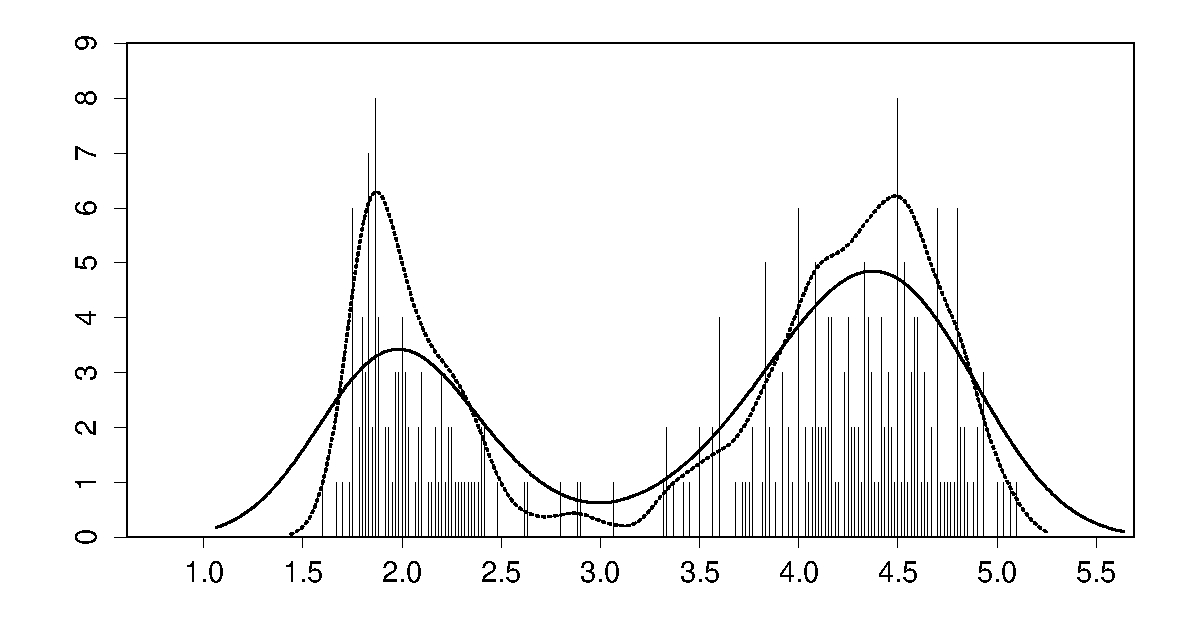
\includegraphics[width=.5\textwidth]{geys-2kern} %<< no file extension
  %%         --- .5\textwidth stands for 50% of text width
  \caption[Geyser data: binned histogram, Silverman's and another
  kernel]%<<-- Legend for the list of figures at the beginning of you thesis
  {Old Faithful Geyser eruption lengths, $n=272$; binned data and two
    (Gaussian) kernel density estimates ($\times 10$) with $h=h^*= .3348$
    and $h= .1$ (dotted).}% legend displayed below the graph.
  \label{fig:geys2}
\end{figure}

\section{To make a proof}
\begin{proof}
  $1 + 1 = 2$
\end{proof}

\section{To include \Rp code}
See information in Appendix~\ref{app:complement}.


\section{Other information}
Put a text between quotes: make sure to use nice quotes, such as ``quote''.

Cite a document in the bibliography (an example here): \cite{Reference}.
%%--> in file   myReferences.bib  (same directory)
Or mention that \citeauthor{HamF85} (a person) or \citeauthor{StaWW91} (two
persons) have already done quite a bit work.

Referencing a different part of your work: please refer to Appendix \ref{app:complement}.


%%% Local Variables: 
%%% mode: latex
%%% TeX-master: "MasterThesisSfS"
%%% End: 

%\include{Chapter...}
\chapter{Summary}
\label{s:Summary}

Summarize the presented work. Why is it useful to the research field or institute?


\section{Future Work}
\label{ss:FutureWork}

Possible ways to extend the work.


%%% Local Variables: 
%%% mode: latex
%%% TeX-master: "MasterThesisSfS"
%%% End: 
 

%%%%%%%%%%%%%%%%%%%%%%%%%%%%%%%%%%%%%%%%%%%%%%%%%%%%%%%%%%%%%%%%%%%%%%%%%%%%%%%
%%%  Bibliography                                                           %%%
%%%%%%%%%%%%%%%%%%%%%%%%%%%%%%%%%%%%%%%%%%%%%%%%%%%%%%%%%%%%%%%%%%%%%%%%%%%%%%%
\addtocontents{toc}{\vspace{.5\baselineskip}}
\cleardoublepage
\phantomsection
\addcontentsline{toc}{chapter}{\protect\numberline{}{Bibliography}}
\bibliography{Mendeley}

%%%%%%%%%%%%%%%%%%%%%%%%%%%%%%%%%%%%%%%%%%%%%%%%%%%%%%%%%%%%%%%%%%%%%%%%%%%%%%%
%%%  Appendices (if needed)                                                 %%%
%%%%%%%%%%%%%%%%%%%%%%%%%%%%%%%%%%%%%%%%%%%%%%%%%%%%%%%%%%%%%%%%%%%%%%%%%%%%%%%
\addtocontents{toc}{\vspace{.5\baselineskip}}
\appendix
\chapter{Complementary information}
\label{app:complement}

Additional material. For example long mathematical derivations could be
given in the appendix. Or you could include part of your code that is
needed in printed form. You can add several Appendices to your thesis (as
you can include several chapters in the main part of your work).

\section{Including \Rp code with verbatim}
A simple (rather too simple, see~\ref{App:listings}) way to include code or
{\it R} output is to use 
\texttt{verbatim}. It just prints the text however it is (including all
spaces, ``strange'' symbols,...) in a slightly different font.
\begin{verbatim}
## loading packages
library(RBGL)
library(Rgraphviz)
library(boot)

## global variables
X_MAX <- 150

   This allows me to put as many s  p a   c es   as I want.
I can also use \ and ` and & and all the rest that is usually only 
accepted in the math mode.

I can also make as 
                  many 
             line 
    breaks as 
I want... and
             where I want. 
\end{verbatim}

\section{Including \Rp code with the \emph{listings} package}\label{App:listings}
However, it is much nicer to use the \emph{listings} package to include \Rp
code in your report. It allows you to number the lines, color the comments
differently than the code, and so on.

\lstinputlisting{images/picture.R}


\section{Using Sweave to include \Rp code (and more) in your report}
The easiest (and most elegant) way to include \Rp code and its output (and
have all your figures up to date with your report) is to use Sweave. You
can find an introduction Sweave in \texttt{/u/sfs/StatSoftDoc/Sweave/Sweave-tutorial.pdf}.

%%% Local Variables: 
%%% mode: latex
%%% TeX-master: "00_Master"
%%% End: 

\chapter{Yet another appendix....}

\section{Description}
\begin{description}
\item[Something] details.
\item[Something else] other definition.
\end{description}

\section{Tables}
Refer to Table~\ref{tab:example} to see a left justified table with caption
on top.

\begin{table}[ht]
\centering
\caption[Test results]{\label{tab:example}Results.}
\begin{tabular}{ll}
\hline
\textbf{Student} & \textbf{Grade}\\
\hline
Marie  & $6$\\
Alain  & $5.5$\\
Josette  & $4.5$\\
Pierre  & $5$\\
\hline
\end{tabular}
\end{table}

%%% Local Variables: 
%%% mode: latex
%%% TeX-master: "MasterThesisSfS"
%%% End: 


%% Epilogue (optional)
\addtocontents{toc}{\vspace{.5\baselineskip}}
\cleardoublepage
\phantomsection
\addcontentsline{toc}{chapter}{\protect\numberline{}{Epilogue}}
\markboth{Epilogue}{Epilogue}
\chapter*{Epilogue}
\label{s:Epilogue}

A few final words.



%%% Local Variables: 
%%% mode: latex
%%% TeX-master: "00_Master"
%%% End: 


%%%%%%%%%%%%%%%%%%%%%%%%%%%%%%%%%%%%%%%%%%%%%%%%%%%%%%%%%%%%%%%%%%%%%%%%%%%%%%%
%%%  Declaration of originality                                             %%%
%%%%%%%%%%%%%%%%%%%%%%%%%%%%%%%%%%%%%%%%%%%%%%%%%%%%%%%%%%%%%%%%%%%%%%%%%%%%%%%
%% fill in the empty document confirmation-originality.pdf electronically
%% print it out and sign it, scan it in again and save the scan to this
%% directory
\cleardoublepage
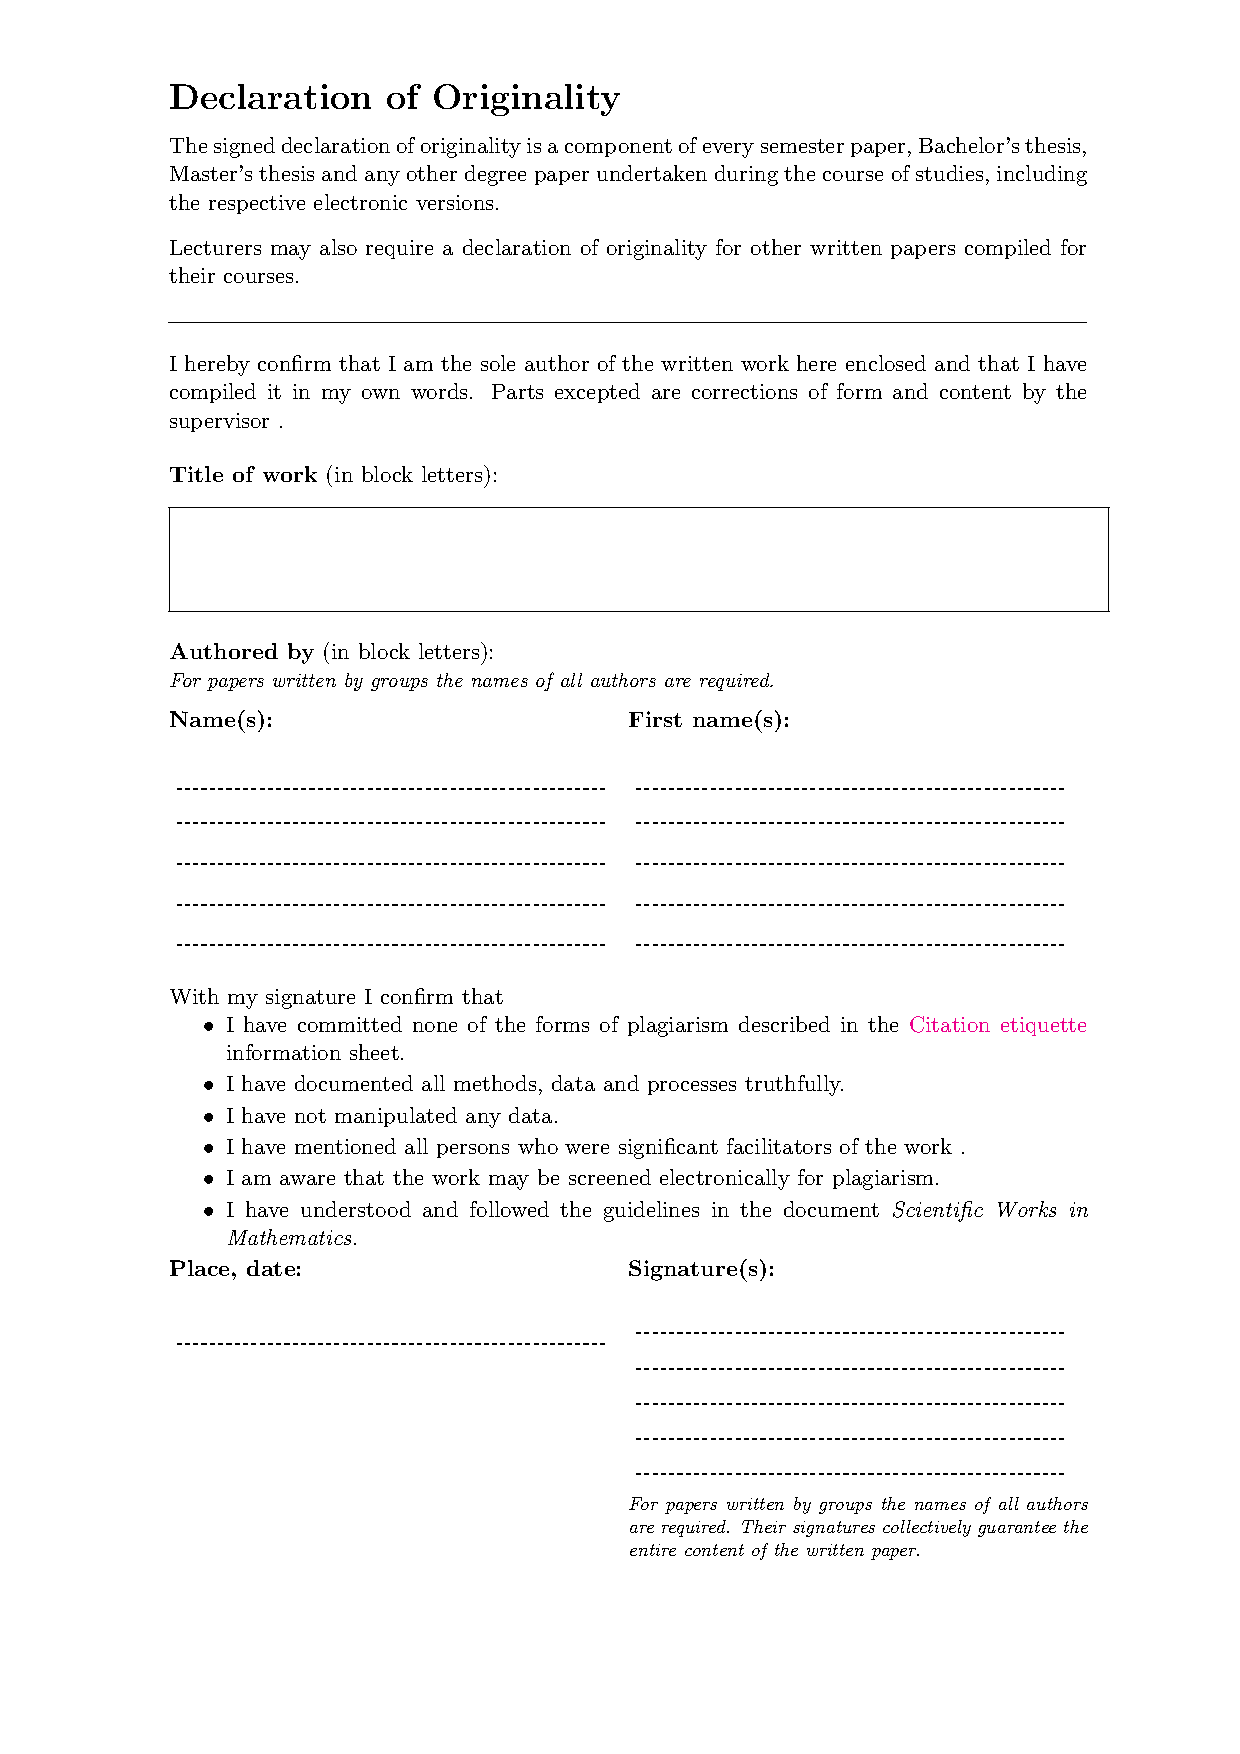
\includepdf[pages={-}, frame=true,scale=1]{34_Originality.pdf}
\end{document}
